
\subsection{Motor Control}
The motors chosen for this project were two small geared DC motors\footnote{ \href{https://www.sparkfun.com/products/13258}{Motors}}.
In order to control them an H-bridge for each of the motors was made using the schematics on figure \ref{fig:hbridge}.


\begin{figure}[H]
\centering
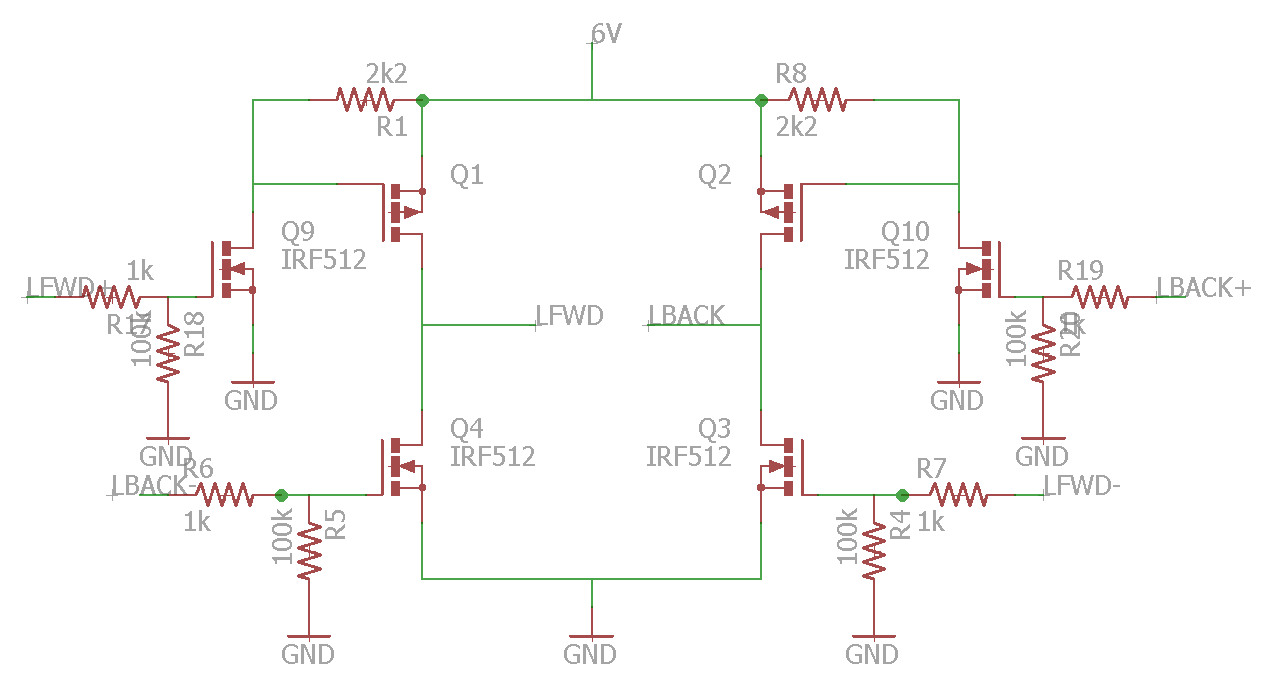
\includegraphics[width = 0.8 \textwidth]{images/hbridge_schematics}
\caption{H-bridge schematics.}
\label{fig:hbridge}
\end{figure}

A full H-bridge is required in order to control the segways movement in both directions such that it is able to both move and recover from a fall when moving around.
Each motor is made with each their separate H-bridge in order to facilitate the rotation of the segway.

In a basic H-bridge, four transistors are used to drive the current on the motor in order to supply the motor with a virtual positive and negative power.
In the case of using MOSFET transistors, it is necessary to use two different voltage levels in the control signal.
This is because the source of the high transistors is connected to the motor, which will induce a certain voltage in the source when the motor is running.
This voltage would automatically disable the MOSFET if the voltage on the gate is not high enough.
Therefore the voltage level of the high control signals should be the same as to the motor voltage to control the MOSFETs.
As the H-bridge is to be controlled with the direct signal from the FPGA, a more complex design is needed.

The H-bridge design in figure \ref{fig:hbridge} gives the possibility of controlling the motors using a 5V supply and a 3.3V control signal.
Using two p-channel MOSFETs in the high part of the driver, it is possible to open and close these MOSFETs by setting their gate to ground or the power supply using a secondary n-channel MOSFET driven with the direct FPGA signal as shown in the schematics on figure \ref{fig:hbridge}.

